\subsection{Motivation for optimisation approach}
Most approaches to designing Bézier polynomial-based virtual constraints for a bipedal robot can be classed in one of three categories; \textit{manual design}, \textit{sampling} or \textit{optimisation}. Manual design involves a human operator producing the control points directly. Sampling is the utilisation of some method of choosing coefficients in an attempt to span the configuration space, either by random selection or gridding. Optimisation approaches choose coefficients which minimise some cost function under particular constraints.

Manual design approaches are not favourable since they are expensive and inefficient in comparison to automatic generation of virtual constraints. Sampling methods, while much faster at generating a single virtual constraint than manual generation, suffer from the \textit{curse of dimensionality}. That is, in order for a sampling method to produce the same density of coverage, the number of samples required increases exponentially with the number of dimensions. Using a brute-force sampling approach produces many redundant primitives which exhibit similar net changes in the mechanical energy of the walker and paths of the end of the swing leg. It is also difficult to ensure that the conditions for feasible walking are met using pure sampling methods.

The redundancy inherent in the sampling approach increases the memory required to store the virtual constraint library and the computational requirements of both its generation and use in real time. An optimisation approach attempts to find the best virtual constraint subject to particular requirements. Therefore, the utility of single virtual constraint optimisation is to avoid the large amount of redundancy involved in the sampling approach and to enable the enforcement of feasible walking conditions.

\subsection{Definition of optimality}
As with most physical systems, there are competing definitions of optimality in the case walking robots \cite{sreenath2011compliant, westervelt2003hybrid, hurmuzlu2004modeling}. The definition of optimality chosen for the purposes of producing the virtual constraint library is as follows:
\emph{The optimal virtual constraint for a given start and end configuration and kinetic energy gain or loss is the one which requires the minimum input energy to maintain.}

We note that the relationship between torque and electrical energy in conventional DC motors is typically approximated by the following equation:
\begin{equation} \label{eqn:motorenergy}
	E(t) \approx \int\limits_0^t u(s)^2 ~ ds
\end{equation}

However, since the partial solution of the zero dynamics is in terms of $\theta$ rather than time, this is not a convenient cost function. Therefore, since we may calculate $\dot{\theta}(\theta)^2$ and by assumption $\theta$ is monotonic ($\dot{\theta}>0$), the cost function
\begin{equation}
	J_\alpha = \int\limits_{\theta_0}^{\theta^-} \left\lVert \frac{u_\alpha(\theta)}{\dot{\theta}(\theta)} \right\rVert_2^2 ~ d\theta
\end{equation}
is used to approximate Equation \ref{eqn:motorenergy} evaluated over the virtual constraint. Note that the L2-norm is included to encapsulate the contribution of multiple torques, since in all but the simplest walking robots, there is more than one actuated joint.

\subsection{Validity of convex optimisation approach}
The decision variables for the purpose of optimisation are the Bézier coefficients $\alpha$. Since the formulation of the cost function $J$ is not linear or quadratic in these decision variables, the optimisation problem becomes more complex; see Section \ref{sec:nonlinopt}. Linear and quadratic techniques are not immediately applicable to the nonlinear case, leaving two alternatives: gridding approaches and nonlinear programming. Gridding approaches in optimisation are subject to the same limitations described above. Indeed, if the advantage of optimisation is to avoid using gridding, then such an approach is clearly a poor choice. However, nonlinear programming will only produce reasonable results under certain conditions.

It is not possible to determine \textit{a priori} that an optimisation is well-formed, that is, will result in a valid solution. Furthermore, for nonlinear optimisation to produce favourable results, the cost function must be convex or near-convex close to the initial estimate. It is therefore of significant interest to determine how close the cost function is to being convex. For the two-link compass gait walker, it is possible to produce such a verification, since we can formulate an optimisation with only two decision variables, which is easily visualised. In Figure \ref{fig:cggridtorque}, we see that gridding the two decision variables produces a surface that appears to be well-behaved and convex. It is reasonable to suggest that this is generalisable to higher degree constraints with more decision variables than for the compass-gait robot.

\begin{figure}
	\centering
	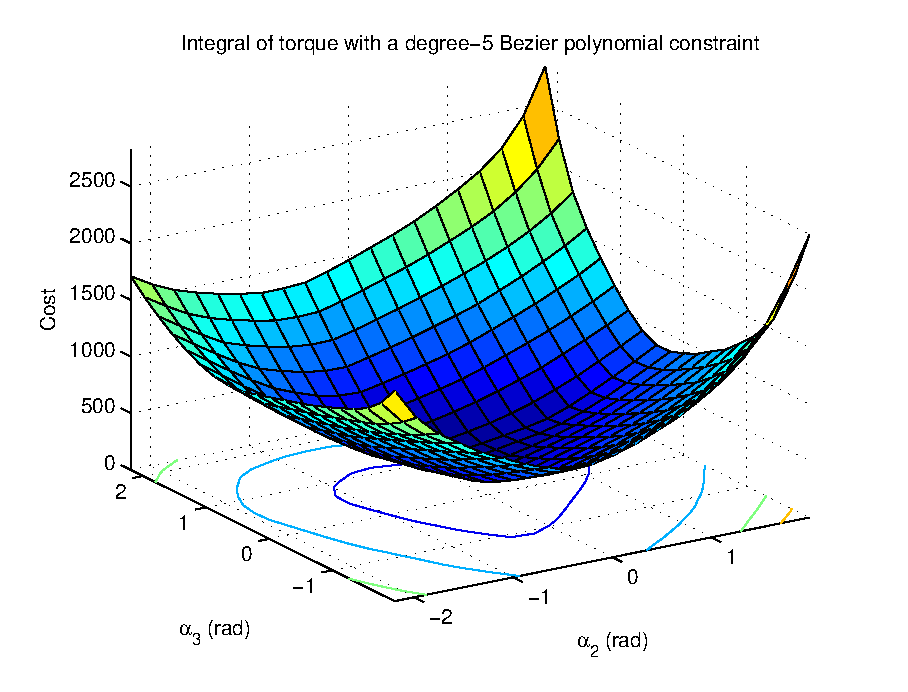
\includegraphics[width=0.6\linewidth]{4VirtConstLib/CGgrid.eps}
	\caption{Cost function of a two decision variable compass-gait optimisation}
	\label{fig:cggridtorque}
\end{figure}

In the case of higher-DOF walking models, it becomes more difficult to confirm near-convexity. Intuition suggests that large decision variables should result in high costs which suggests that the overall behaviour should be somewhat well behaved, however this must be verified. Taking slices, where we choose two decision variables over which to grid and fix all others, may provide some basis for verifying that the result for the compass-gait is generalisable to higher degree of freedom walkers. This is deferred to a later work.

\subsection{Optimisation method} \label{sec:optmethod}
\subsubsection{Decision variables and constraints}
While the objective of single constraint optimisation is to produce an optimum VC independent of any other virtual constraints in the library, it is important to formulate the optimisation problem in a manner which enables a useful library to be produced. The motion primitive library is intended to contain VCs which span the configuration space of the robot's natural walking as well as including a range of mechanical energy additions and subtractions to facilitate walking over uneven terrain. Therefore, it seems clear that each single constraint optimisation should be formulated subject to constraints on the start and end configurations of the footstep, along with a prescribed energy gain or loss. In addition, it is necessary to specify the ground height applicable to the virtual constraint, since a feasible step cannot intersect with the ground between the start and end conditions.

Since the potential energy change is prescribed by the start and end conditions, it is convenient to formulate the optimisation using kinetic, rather than total mechanical, energy. The change in kinetic energy $\Delta$KE from one footstep to the next could be calculated with respect to numerous reference points. A simple and obvious choice is to define $\Delta$KE as the change in kinetic energy from $\theta_0 \rightarrow \theta^+$.

The ground height at a horizontal displacement $x$ from the end of the stance leg is encoded in the scalar function $\sigma(x)$. For the purposes of analysing a virtual constraint, the ground height is pertinent only when considering the end of the swing leg, thus we may produce a more convenient representation $\sigma(\theta)=\sigma(p_h(\theta))$. The ground height places the following nonlinear constraints on the optimisation:
\begin{equation} \label{eqn:groundheight}
	p_v(\theta) \left\{
	\begin{array}{lcr}
		= \sigma(\theta) &:& \theta \in \{\theta_0, \theta^-\} \\
		> \sigma(\theta) &~& \mathrm{otherwise}
	\end{array} \right.
\end{equation}

Recall from Section \ref{sec:bezconstraints} that in order to be physically realisable, a VC must satisfy several conditions. The \textit{invariance conditions}, \ref{item:configinvariance} and \ref{item:velinvariance}, place restrictions on the admissibility of a primitive on the basis of the VC which precedes it. The first condition is not of great concern in the construction of a single primitive, since the responsibility of ensuring coverage of start and final configurations is deferred to the library generation. However, it is important to consider the latter condition when generating a single constraint; in order for the library to be useful, any VC which matches the prior primitive through the impact map should be a valid choice of successor. This implies that the slope of all constraints at the end point for any given final configuration ought to be identical. A reasonable choice to satisfy this condition is to enforce that the final slope must be zero for all constraints. This has the additional advantage of making the constraints more robust to errors in ground height perception. Note that this simplifies the compliance of virtual constraints to \ref{item:frictioncone}. With zero final slope enforced, a final configuration $q^-$ is valid only if 
\begin{equation} \label{eqn:zeroslopefriccone}
	\left\lvert \frac{(\Delta_F(q^-))_{1,n}}{(\Delta_F(q^-))_{2,n}}\right\rvert < \mu_s
\end{equation}

When formulating an optimisation, it is advantageous to minimise the number of decision variables, if all else is considered static, since this reduces the evaluation time. This is particularly true for variables which are subject to constraints. It is notable that fixing the start and end configuration of the constraint along with enforcing zero slope at the final configuration fixes the four outermost columns of $\alpha$. As such, we consider these fixed and exclude them as decision variables. The optimisation variables therefore take the form given in Table \ref{tab:optDecVars}. Note that the conditions in Section \ref{sec:bezconstraints} along with the equality constraint in Equation \ref{eqn:groundheight} are all concerned with those four outermost columns of $\alpha$, therefore in the single VC optimisation, these conditions are not applicable.

\begin{table}
	\centering
	\begin{tabular}{c | c | c | c}
		            Variable             & Generated                     & Decision Variable & Opt constraint \\ \hline
		   $\theta_0$ and $\theta^-$     & From start/end condition      & No                & No             \\
		   $\alpha_0$ and $\alpha_N$     & From start/end condition      & No                & No             \\
		         $\alpha_{N-1}$          & Set to $\alpha_N$             & No                & No             \\
		           $\alpha_1$            & From \ref{item:velinvariance} & No                & No             \\
		$\alpha_2, \ldots, \alpha_{N-2}$ & Optimisation                  & \textbf{Yes}      & No             \\
		           $\Delta$KE            & Supplied                      & No                & \textbf{Yes}   \\
		          $\sigma(x)$            & Supplied                      & No                & \textbf{Yes}
	\end{tabular}
	\caption{Variables involved in the single VC optimisation}
	\label{tab:optDecVars}
\end{table}

\subsubsection{Nominal initial velocity}
The torque required to maintain a virtual constraint is not only dependent on the configuration path, but also the velocity. VCs prescribe the configuration path and constrain the velocity to be a function of the initial phase variable velocity. As a result, the torque required to maintain a virtual constraint is a function of the initial velocity. In addition, $\Delta$KE is affine in the square of the initial phase variable velocity. It is therefore necessary to formulate a \textit{nominal initial velocity}, $\dot{\theta}_\alpha^*$. We assume that in practice, the constraint will be chosen with initial velocities close to $\dot{\theta}_\alpha^*$ and should therefore be near-optimal. Under that assumption, the change in kinetic energy should be close to the prescribed $\Delta$KE, however this is less important since setting $\Delta$KE is in service of producing a rich library.

Choosing a nominal velocity for each constraint is non-trivial. It should be noted that the choice of nominal velocity significantly influences the optimisation. Choosing a single $\dot{\theta}^*$ for all VCs is not appropriate, each virtual constraint may differ in the minimum velocity required to complete the motion. It seems necessary to treat the constraints separately based upon the desired $\Delta$KE and minimum initial velocity $\dot{\theta}^c_\alpha$.

For \textbf{energy-additive constraints}, for which $\Delta$KE $>0$, the key issue of importance is that the virtual constraint itself is feasible, since the next primitive will have additional kinetic energy. Therefore, we set the initial velocity such that $\dot{\theta}_\alpha^* = \lambda\dot{\theta}_\alpha^c$, where $\lambda$ is some fixed ``factor of safety'':
\begin{equation} \label{eqn:energyadditive}
\dot{\theta}_{\alpha,\Delta\mathrm{KE}^+}^{*^2} = -\lambda^2\frac{ \Psi_\alpha(\theta_\alpha^c)}{ \Gamma_\alpha(\theta_\alpha^c)}
\end{equation}

For \textbf{energy-subtractive constraints}, for which $\Delta$KE $<0$, assuming that the robot should never come to a stop or fall back, the energy reduction should result in further constraints being feasible. In order to avoid using any data external to the constraint, we use the value of $\dot{\theta}_\alpha^c$ associated with the same VC. This is reasonable, particularly if the constraint is operating over terrain which has a systematic structure over greater distances than the step length, e.g. a long downward slope. The post impact velocity is calculable with $\Delta_\alpha$ as defined in Equation \ref{eqn:Delthd}:
\begin{subequations}
	\begin{align}
	\dot{\theta}^{-^2} &= \Gamma_\alpha(\theta_\alpha^-)\dot{\theta}_\alpha^{*^2} + \Psi_\alpha(\theta_\alpha^-) \\
	\dot{\theta}^+ &= c\Delta_\alpha\dot{\theta}^-
	\end{align}
\end{subequations}
Equating $\dot{\theta}^+$ with $\lambda\dot{\theta}_\alpha^c$, where $\lambda$ is the same factor of safety as in Equation \ref{eqn:energyadditive}:
\begin{equation}
	\dot{\theta}_{\alpha,\Delta\mathrm{KE}^-}^{*^2} = \frac{(c\Delta_\alpha)^{-2}\left(-\lambda^2\frac{ \Psi(\theta_\alpha^c)}{ \Gamma(\theta_\alpha^c)}\right) - \Psi(\theta_\alpha^-)} {\Gamma(\theta_\alpha^-)}
\end{equation}

\textbf{Energy-neutral constraints} result in $\Delta$KE $=0$. In this case, we expect the next constraint to require an initial $\dot{\theta}$ no greater or less than $\dot{\theta}_\alpha^*$. As such, either of the above expressions seem suitable. The simplicity of Equation \ref{eqn:energyadditive} is preferred.

\subsection{Implementation}
The \mcode{optimiseVC} function takes as arguments the start and end configurations of the constraint, the desired change in kinetic energy, the ground definition $\sigma(x)$ and the degree of the desired Bézier polynomial. It returns the start and end values of the phase variable $\theta_0$, $\theta^-$ and the Bézier coefficients $\alpha$, along with the calculated values of the partial solution at $\theta_c$, $\theta^-$ and $\theta^+$.

The single VC implementation is achieved using MATLAB's constrained nonlinear programming function \mcode{fmincon}. This uses an interior point method to seek local minima in the cost function subject to the given constraints. For each set of test values for the decision variables, the partial solution ($\Gamma(\theta)$ and $\Psi(\theta)$) is evaluated by producing a grid of $\theta$ values in $[\theta_0, \theta^-]$. The cost is calculated using trapezoidal integration on the resulting torque values. Since $\Delta$KE also relies upon the partial solution, it is held persistently in a helper function and only recalculated upon differing decision variables, to avoid inefficient recalculation.

The desired $\Delta$KE is implemented in the optimisation as a nonlinear inequality constraint. That is, for each iteration of \mcode{fmincon}, the change in kinetic energy under the virtual constraint $\Delta\mathrm{KE}_{act}=\mathrm{KE}(\theta^+)-\mathrm{KE}(\theta_0)$ is calculated. \mcode{fmincon} is configured such that it attempts to uphold $\Delta\mathrm{KE}-\Delta\mathrm{KE}_{act}\leq 0$. An inequality constraint was used because this is better conditioned than an equality constraint for the numerical optimisation method; using an equality constraint results in a longer computation time and an increased chance of infeasibility. It is reasonable to expect that the resulting kinetic energy mutation should closely match the desired, since adding more kinetic energy typically requires more torque. In cases where kinetic energy is subtracted, this is less certain, however it holds true as long as the desired energy subtraction is smaller than that achieved through the impact or by stepping up.

$\sigma(x)$ is defined by specifying the ground height at individual points. From this, the ground level over all $x$ is determined by a zero-order hold. The ground constraint is enforced by taking relatively sparse samples from $\theta_0$ to $\theta^-$ and testing for each sample that $p_v(\theta)>\sigma(\theta)$. A natural choice of samples is at each Bézier control point, such that the sampling of the ground is dependent on the degree of the polynomial. It is reasonable to test only several points along the trajectory on the assumption that the ground height changes at relatively few points over one footstep and that the swing leg traces a smooth arc between its start and end points. The second assumption is valid for all physical robots. The first is able to be justified by the design of the library generation. In the case of the compass-gait robot, due to its morphological simplicity, the $\sigma(x)$ constraint is not applied. Indeed, it is not possible for the compass-gait robot to complete walking motion on flat ground without scuffing its swing leg if no means are provided to shorten it.

It is necessary to avoid very large Bézier coefficients, where $\alpha(\theta)$ crosses zero many times over the interval $[\theta_0, \theta_f]$ (see Section \ref{sec:alphazerocrossing}). This may be achieved by regularisation \cite{seidman1989well}, boundary functions on $\alpha(\theta) = 0$ or simple bounds on the admissible values of the coefficients. Regularisation was used to produce the results of this thesis due to its efficacy in both improving the convexity of the cost function and therefore the convergence of the minimisation as well as avoiding $\alpha(\theta)$ zero crossings, which occur with increased coefficient values. 

Regularisation adds some cost based on the values of the decision variables. For the purposes of this optimisation, the cost was simply a constant times the 2-norm of the Bézier coefficients, producing a cost function of the form
\begin{equation} \label{eqn:regcost}
J^* = \int_{\theta_0}^{\theta^-}\left\lVert u_\alpha(\theta) \right\rVert_2^2 ~ d\theta
+ \lambda\left\lVert \alpha \right\rVert_2
\end{equation}
This penalises virtual constraints if they have $\alpha_i$ values distant from 0. Zero is a reasonable choice for the centre of the regularisation cost, since the values of the coefficients for useful constraints are typically small. A more complicated but perhaps better choice could be to penalise the divergence from the line in the Bézier coordinate space between the start and endpoint, however in practice this should not make a significant difference so long as $\lambda$ is kept small compared to $J$.

In summary, the nonlinear optimisation is formulated as such:

\textbf{Cost}: Squared L2-norm of torque plus regularisation

\textbf{Nonlinear inequality constraints}: End of swing leg is above ground level except at impacts (other than for the 2-link compass-gait), and the achieved $\Delta$KE is greater than or equal to the desired energy change.

\subsection{Coping with zero crossings of $\alpha(\theta)$} \label{sec:alphazerocrossing}
Recall from Section \ref{sec:partialsol} that we assume that $\alpha(\theta)\neq 0$ in order to derive the partial solution (Equation \ref{eqn:affinesoln}). This is an important assumption to make, since if at any point $\theta \in [\theta_0, \theta^-], \alpha(\theta) = 0$, the terms $\frac{\beta(\theta)}{\alpha(\theta)}$ and $\frac{\gamma(\theta)}{\alpha(\theta)}$ are undefined. In principle, this is not a significant problem; the partial solution still exists and is correct for all $\theta \not \in \Theta_z$, where $\Theta_z$ is the set of $\theta \in [\theta_0, \theta^-]$ for which $\alpha(\theta)=0$ \cite{shiriaev2005constructive}.

Unfortunately, $\alpha(\theta)$ may cross zero, particularly in primitives which have the robot completing what may be termed ``exaggerated'' motion. Consider Figure \ref{fig:alphazerocrossing}: $\alpha(\theta)$ dips below zero in a constraint where the swing leg crosses the horizontal and points skyward. In the general case, there may be an unbounded number of zero crossings of $\alpha(\theta)$.

\begin{figure}
	\centering
	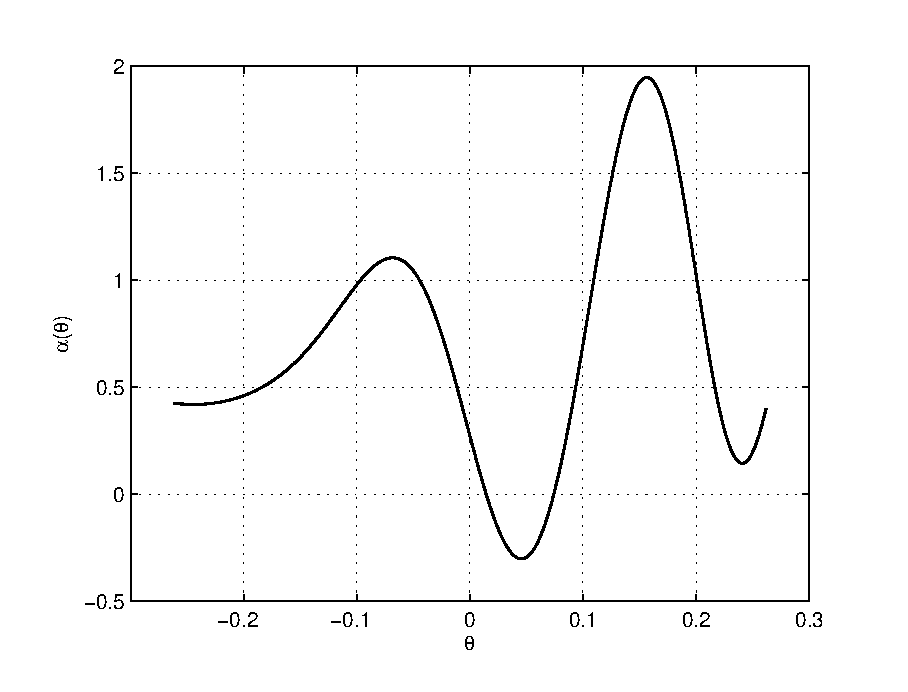
\includegraphics[width=0.49\linewidth]{4VirtConstLib/al0Crossing.eps}
	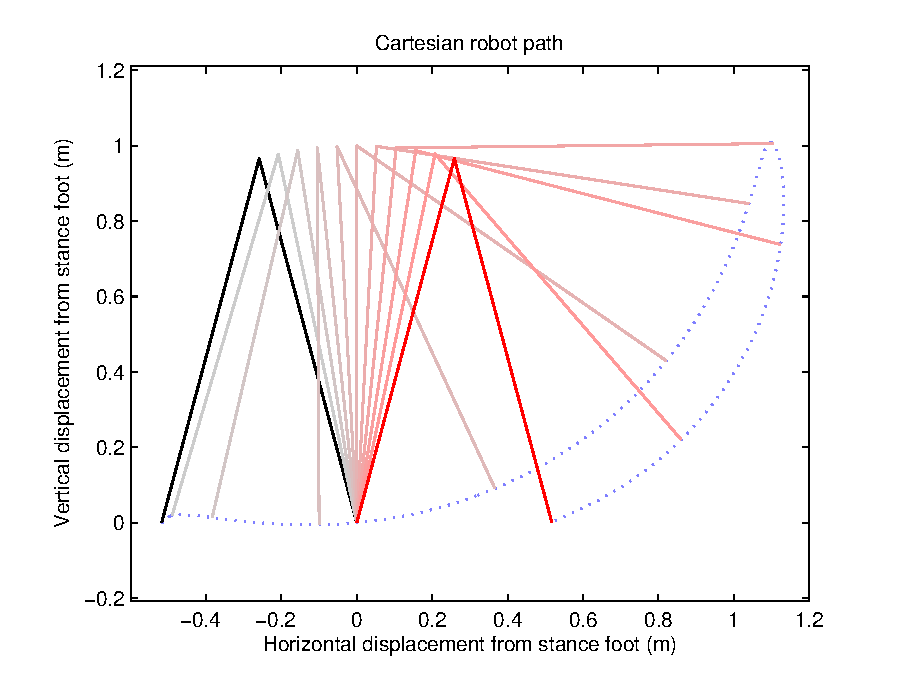
\includegraphics[width=0.49\linewidth]{4VirtConstLib/xy-0Crossing.eps}
	\caption{Zero crossing of $\alpha(\theta)$ for compass-gait robot}
	\label{fig:alphazerocrossing}
\end{figure}

By virtue of the sampling approach to solving the partial solution (see Appendix \ref{app:partialsol} for details), there is a vanishingly small chance of sampling exactly at the point where $\alpha(\theta)=0$. This is not the concern; when $\alpha(\theta)$ is close to zero, the terms in the differential equation diverge, thus the values of the partial solution and therefore the torque are very sensitive to the relative position of the zero crossing to the sampling interval. This may compromise the convexity of the cost function. Figure \ref{fig:divergence0crossing} demonstrates the erroneous solution obtained by uniform sampling over $[\theta_0, \theta^-]$.
 
\begin{figure}
	\centering
	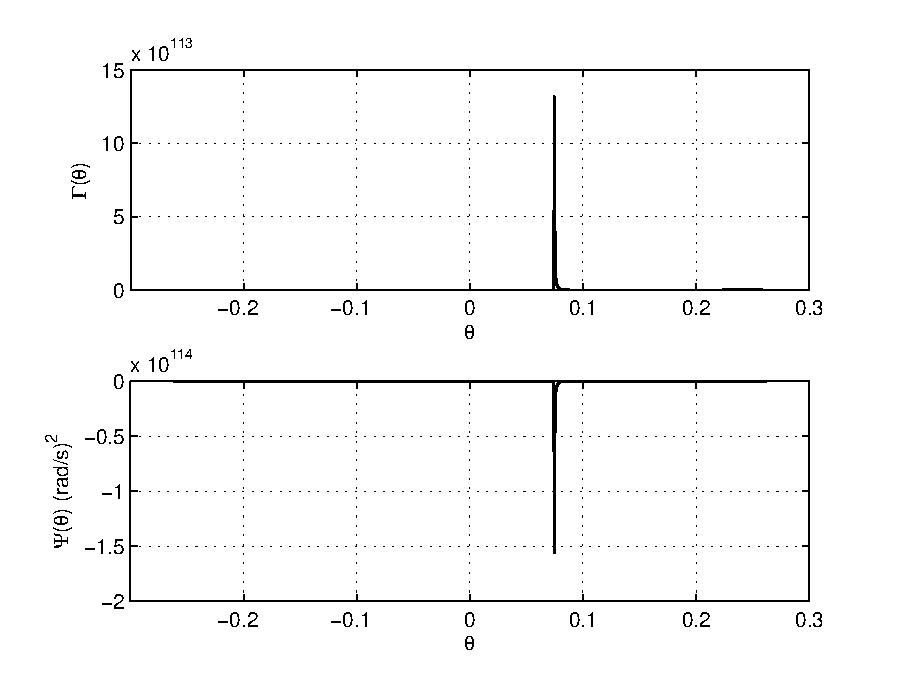
\includegraphics[width=0.6\linewidth]{4VirtConstLib/GamPsi0Crossing.eps}
	\caption[Irregular behaviour of $\Gamma(\theta)$ and $\Psi(\theta)$ with zero crossings of $\alpha(\theta)$]{Irregular behaviour of $\Gamma(\theta)$ and $\Psi(\theta)$ with zero crossings of $\alpha(\theta)$ using uniform sampling}
	\label{fig:divergence0crossing}
\end{figure}

%\begin{figure}
%	\centering
%	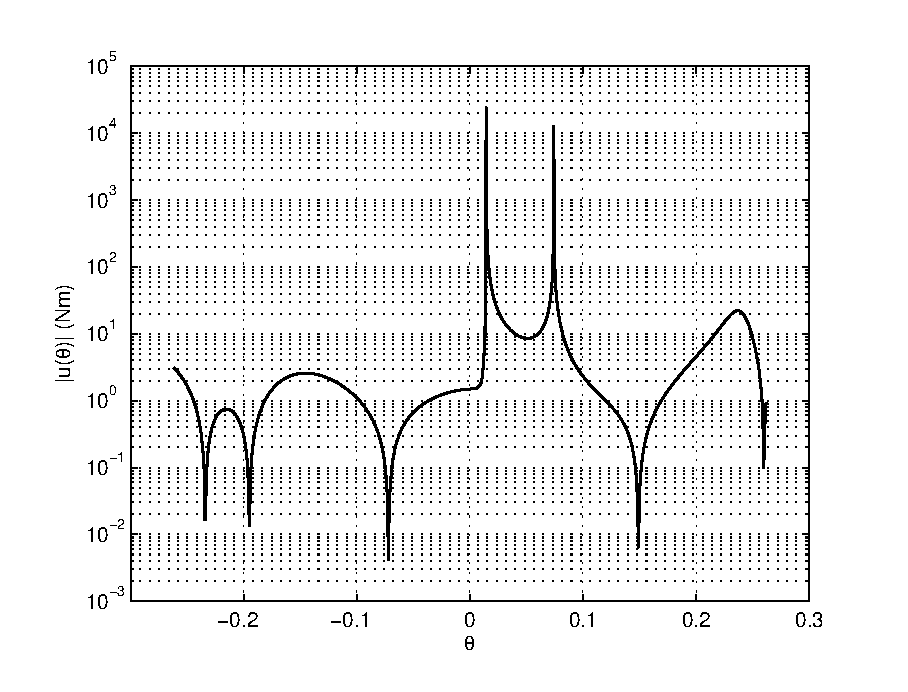
\includegraphics[width=0.6\linewidth]{4VirtConstLib/u-0Crossing}
%	\caption[Absolute value of torque with zero crossings of $\alpha(\theta)$]{Absolute value of torque with a zero crossings of $\alpha(\theta)$ based upon uniform sampling}
%	\label{fig:bad0crossingtorque}
%\end{figure}

It is necessary to alter the method of calculating the partial solution if $\alpha(\theta)$ crosses zero; the interval $[\theta_0, \theta^-]$ must be divided at every zero crossing of $\alpha(\theta)$ and the integration must be performed only over those intervals. Due to the sensitivity of the solution to the exact location of the zero crossing on the sampling interval (which is not improved by finer sampling), it is necessary to locate the zero crossing and to ensure that the sampling is symmetrical nearby. This method may be called \textit{adaptive sampling}. Figures \ref{fig:betterGamPsi} and \ref{fig:bettertorque} demonstrate the significant improvements in the behaviour of the numerical solutions gained by using this method. Note that, unlike in Figure \ref{fig:divergence0crossing}, there is no residual effect of the divergence in $\Gamma(\theta)$ and $\Psi(\theta)$.

\begin{figure}
	\begin{minipage}{0.48\textwidth}
		\centering
		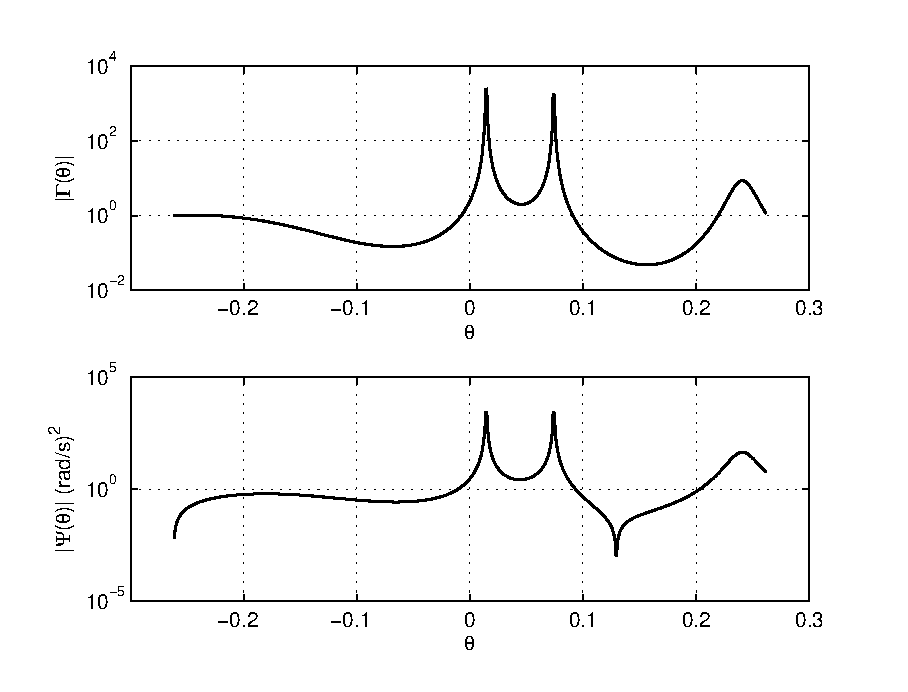
\includegraphics[width=\linewidth]{4VirtConstLib/betterGamPsi}
		\caption{Improvements to partial solution using adaptive sampling}
		\label{fig:betterGamPsi}
	\end{minipage}
	\hfill
 	\begin{minipage}{0.48\textwidth}
 		\centering
	 	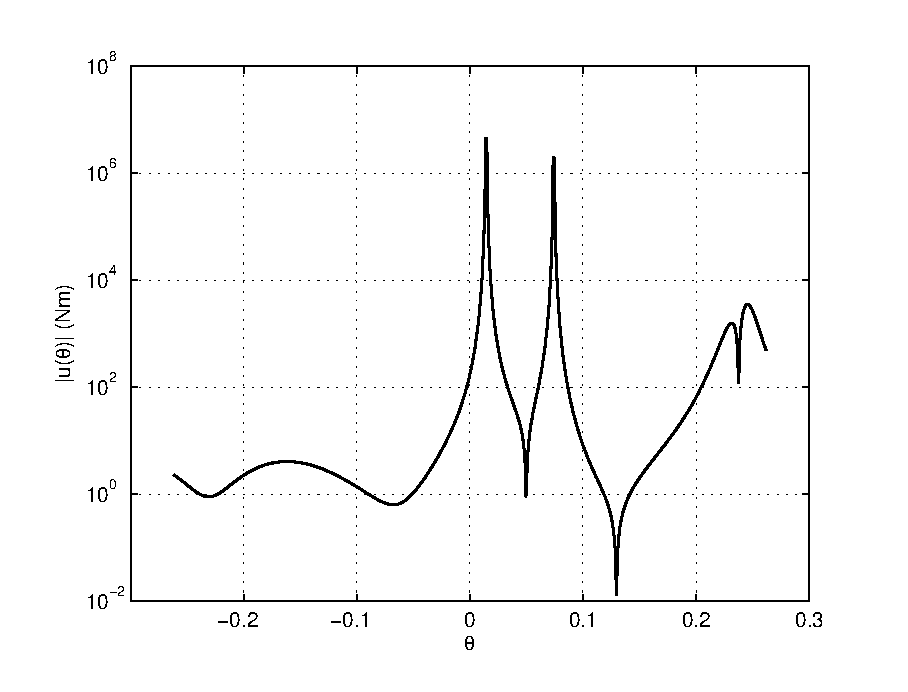
\includegraphics[width=\linewidth]{4VirtConstLib/betterTorque}
	 	\caption[Torque using adaptive sampling]{Torque using adaptive sampling. Note that it is still impulsive}
	 	\label{fig:bettertorque}
 	\end{minipage}
\end{figure}
  
Note that in Figure \ref{fig:bettertorque}, the torque is still much too high for a practicable constraint. This is not a problem; the optimisation is concerned with the value of the cost function, not the physical realisability of the constraints. The improved behaviour of the partial solution attained through the use of adaptive sampling methods is in service of ensuring the cost function remains convex such that a minimum can be found.

Note that this method is flawed where zero crossings occur very close to one another. There is no method of rectifying this other than increasing the sampling density. This is intuitively clear; in order to resolve two zero crossings which merge at low sampling rates, the resolution must be increased. This can be considered analogous to resolving two targets using sensing methods.

It is particularly notable that, for very large values of the Bézier coefficients, $\alpha(\theta)$ becomes very oscillatory, crossing zero many times in the interval $\theta\in[\theta_0, \theta^-]$. A sample of this behaviour, with coefficients possessing values in excess of 200, is presented in Figure \ref{fig:badalpha}. There is no good method of dealing with this behaviour other than avoidance.
  
\begin{figure}
\centering
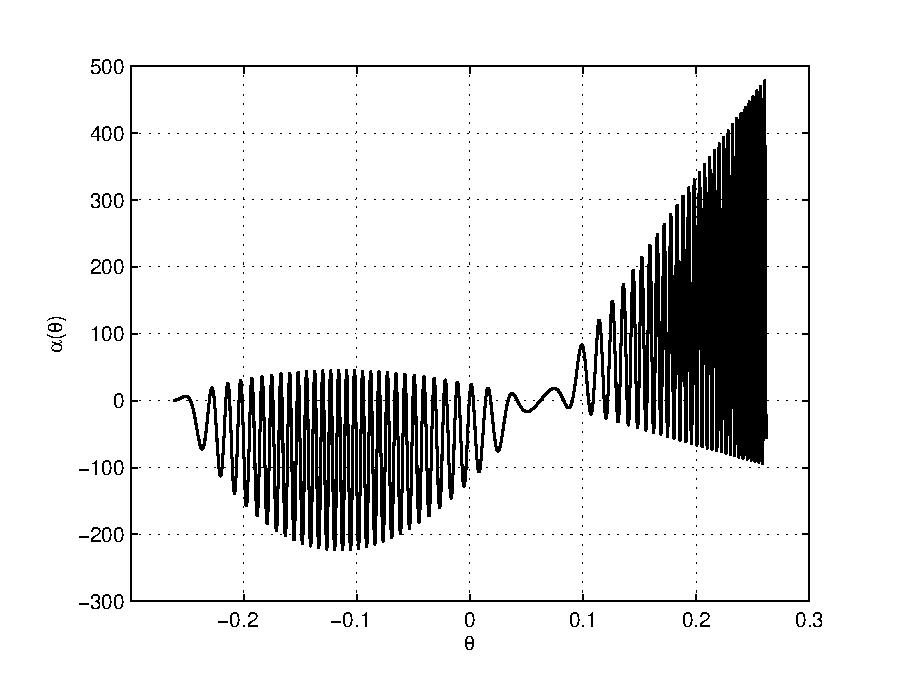
\includegraphics[width=0.6\linewidth]{4VirtConstLib/badalpha}
\caption{Poor behaviour of $\alpha(\theta)$ with very large Bézier coefficients}
\label{fig:badalpha}
\end{figure}
